% !TeX root = ../report.tex
\chapter{Grundlagen}

Im vorliegenden Bericht wird vielseitig auf praktische Aspekte die zum Bau eines Passivradars notwendig sind eingegangen. Um dem Leser das Verständnis dieser Aspekte zu erleichtern, ist es sinnvoll, zunächst die theoretischen Grundlagen zu erläutern. Dieses Kapitel dient der Beschreibung einiger essenzieller Prinzipien, die bei Passivradar zum Einsatz kommen. Dazu wird zunächst der Begriff der bistatischen Geometrie eingeführt und erklärt, anschließend wird diese im Zusammenhang mit passiver Zieldetektion und -lokalisierung kombiniert und mit einer mathematischen Beschreibung versehen. Schließlich wird auf konstruktionsabhängige Eigenarten, sowie Vor- und Nachteile eingegangen.

\section{Bistatische Geometrie}\label{sct:bistatic_geometry}

In der Ortungstechnik versteht man unter dem Begriff der bistatischen Geometrie die räumliche Trennung zwischen einem Sender und einem Empfänger. Bezogen auf Systeme mit mehreren Sendern und Empfängern wird auch der Begriff des multistatischen Systems genutzt. Im umgekehrten Fall, wenn die räumliche Trennung zwischen Sender und Empfänger als vernachlässigbar klein verstanden wird, spricht man von monostatischen Systemen. Die Abbildung~\ref{fig:mono_bi_multistatic_geometry} zeigt vereinfachte Illustrationen dieser Konzepte. Tx und Rx bezeichnen hierbei jeweils Sender und Empfänger im System. Zu beachten hierbei sind die verschiedenen Signalpfade die sich aus der Anordnung der Sender und Empfänger ergeben. Man unterscheidet zwischen Direkt- und Echosignalen, also jeweils solche die auf direktem Wege von Sender zu Empfänger wandern und solche die erst an einem oder mehreren Objekten reflektieren und dann beim Empfänger eingehen. Letztere werden weiter untereteilt in erwünschte (Ziele, engl.\ Targets) und unerwünschte (engl.\ Clutter) Echos.

\begin{figure}[htb]
    \centering
    \subcaptionbox{Monostatische Geometrie.\label{fig:monostatic_geometry}}{
        \begin{tikzpicture}
            \node at (0,0) [draw,fill=white] (radar) {Tx \& Rx};

            \node [label={above:Ziel}] (target) at (2,2) {\Huge\faPlane};

            \draw [<->,red] (radar) -- (target);
        \end{tikzpicture}
    }
    \subcaptionbox{Bistatische Geometrie.\label{fig:bistatic_geometry}}{
        \begin{tikzpicture}
            \coordinate (rx1_coord) at (-1,0);
            \coordinate (tx1_coord) at (2,0);
            \coordinate (target_coord) at (1.75,1.5);

            \node at (tx1_coord) [draw,fill=white] (tx1) {Tx};
            \node at (rx1_coord) [draw,fill=white] (rx) {Rx};

            \node at (target_coord) [label={above:Ziel}] (target) {\Large\faPlane};

            \draw [->,color=red] (tx1) -- (target);
            \draw [->,color=red] (target) -- (rx);
            \draw [->,color=blue] (tx1) -- (rx);
        \end{tikzpicture}
    }
    \subcaptionbox{Multistatische Geometrie.\label{fig:multistatic_geometry}}{
        \begin{tikzpicture}
            \coordinate (rx1_coord) at (-2,1);
            \coordinate (rx2_coord) at (-1,-0.5);
            \coordinate (tx1_coord) at (3,0);
            \coordinate (tx2_coord) at (2,-1);
            \coordinate (target_coord) at (2,2);

            \node at (tx1_coord) [draw,fill=white] (tx1) {Tx 1};
            \node at (tx2_coord) [draw,fill=white] (tx2) {Tx 2};
            \node at (rx1_coord) [draw,fill=white] (rx1) {Rx 1};
            \node at (rx2_coord) [draw,fill=white] (rx2) {Rx 2};

            \node at (target_coord) [label={above:Ziel}] (target) {\Large\faPlane};

            \draw [->,color=red] (tx1) -- (target);
            \draw [->,color=red] (tx2) -- (target);
            \draw [->,color=red] (target) -- (rx1);
            \draw [->,color=red] (target) -- (rx2);
            \draw [->,color=blue] (tx1) -- (rx1);
            \draw [->,color=blue] (tx1) -- (rx2);
            \draw [->,color=blue] (tx2) -- (rx1);
            \draw [->,color=blue] (tx2) -- (rx2);
        \end{tikzpicture}
    }

    \caption{Mono-, Bi- und Multistatische Geometrie.}\label{fig:mono_bi_multistatic_geometry}
\end{figure}

Ein weiterer wichtiger Begriff im Zusammenhang mit bistatischer Geometrie ist die bistatische Entfernung. Malanowski definiert diese in~\cite[S.~10]{Malanowski2019} wie folgt:

\begin{equation}
    R = R_1 + R_2 - R_\text{b}
\end{equation}\label{eq:bistatic_range}

Wobei \(R_\text{b}\) die Strecke des Direktpfades bezeichnet. Die Terme \(R_1\) und \(R_2\) bezeichnen jeweils die Strecke vom Sender zum Ziel und vom Ziel zum Empfänger. Zusammen wird \(R_1 + R_2\) auch als bistatische Summe bezeichnet. Bildlich gesprochen versteht man under bistatischer Entfernung die zusätzliche Strecke die das Echosignal gegenüber dem Direktsignal zurückgelegt hat. Abbildung~\ref{fig:bistatic_range} zeigt diesen Zusammenhang grafisch.

\begin{figure}[htb]
    \centering
    \subcaptionbox{Bistatische Geometrie.\label{fig:bistatic_range_model}}{
        \begin{tikzpicture}
            \coordinate (rx1_coord) at (-2,0);
            \coordinate (tx1_coord) at (2,0);
            \coordinate (target_coord) at (1.75,2);

            \node at (tx1_coord) [draw,fill=white] (tx1) {Tx};
            \node at (rx1_coord) [draw,fill=white] (rx) {Rx};

            \node at (target_coord) [label={above:Ziel}] (target) {\Large\faPlane};

            \draw [->,color=red] (tx1) -- (target) node [black,midway,right] {$R_1$};
            \draw [->,color=red] (target) -- (rx) node [black,midway,above left] {$R_2$};
            \draw [->,color=blue] (tx1) -- (rx) node [black,midway,below] {$R_\text{b}$};
        \end{tikzpicture}
    }
    \subcaptionbox{Bistatische Entfernung.\label{fig:bistatic_range_equation}}{
        \begin{tikzpicture}
            \coordinate (rx1_coord) at (-2,0);
            \coordinate (tx1_coord) at (2,0);
            \coordinate (target_coord) at (1.75,2);

            \draw [dotted,color=gray]
            let
            \p1=($(tx1_coord)-(target_coord)$),
            \p2=($(target_coord)-(rx1_coord)$),
            \p3=($(tx1_coord)-(rx1_coord)$),
            \n1={veclen(\x1,\y1)},
            \n2={\n1+veclen(\x2,\y2)},
            \n3={\n2-veclen(\x3,\y3)}
            in
            (\n1,0) edge node [black,midway,right,align=center] {$+$} (\n1,-1)
            (\n2,-1) edge node [black,midway,right,align=center] {$-$} (\n2,-2)
            (\n3,-2) edge node [black,midway,right,align=center] {$=$} (\n3,-3);

            \draw [->,color=red]
            let
            \p1=($(tx1_coord)-(target_coord)$),
            \n1={veclen(\x1,\y1)}
            in
            (0,0) -- node [black,midway,above,align=center] {$R_1$} (\n1,0);
            \draw [->,color=red]
            let
            \p1=($(tx1_coord)-(target_coord)$),
            \p2=($(target_coord)-(rx1_coord)$),
            \n1={veclen(\x1,\y1)},
            \n2={\n1+veclen(\x2,\y2)}
            in
            (\n1,-1) -- node [black,midway,above,align=center] {$R_2$} (\n2,-1);
            \draw [->,color=blue]
            let
            \p1=($(tx1_coord)-(target_coord)$),
            \p2=($(target_coord)-(rx1_coord)$),
            \p3=($(tx1_coord)-(rx1_coord)$),
            \n1={veclen(\x1,\y1)},
            \n2={\n1+veclen(\x2,\y2)},
            \n3={\n2-veclen(\x3,\y3)}
            in
            (\n2,-2) -- node [black,midway,above,align=center] {$R_{\text{b}}$} (\n3,-2);

            \draw [->,color=green]
            let
            \p1=($(tx1_coord)-(target_coord)$),
            \p2=($(target_coord)-(rx1_coord)$),
            \p3=($(tx1_coord)-(rx1_coord)$),
            \n1={veclen(\x1,\y1)},
            \n2={\n1+veclen(\x2,\y2)},
            \n3={\n2-veclen(\x3,\y3)}
            in
            (0,-3) -- node [black,midway,above,align=center] {$R$} (\n3,-3);
        \end{tikzpicture}
    }
    \caption{Grafische Herleitung der bistatischen Entfernung.}\label{fig:bistatic_range}
\end{figure}

Weitere Einsicht bietet die kartesische Betrachtung der bistatischen Entfernung. Ausgehend vom zweidimensionalen Fall werden zunächst Sender, Empfänger und Ziel kartesischen Koordinaten zugewiesen. Es gelten für die Position des Senders \(\boldsymbol{p}_\text{tx} = \begin{bmatrix} x_\text{tx}, y_\text{tx} \end{bmatrix}\), für die Position des Empfängers \(\boldsymbol{p}_\text{rx} = \begin{bmatrix} x_\text{rx}, y_\text{rx} \end{bmatrix}\) und die Position des Ziels \(\boldsymbol{p} = \begin{bmatrix} x, y \end{bmatrix}\). Dafür ergibt sich für die Entfernungen

\begin{equation}
    R_1 = {\lVert \boldsymbol{p} - \boldsymbol{p}_\text{tx} \rVert}_2 = \sqrt{{(x - x_\text{tx})}^2 + {(y - y_\text{tx})}^2}
\end{equation}
\begin{equation}
    R_2 = {\lVert \boldsymbol{p} - \boldsymbol{p}_\text{rx} \rVert}_2 = \sqrt{{(x - x_\text{rx})}^2 + {(y - y_\text{rx})}^2}
\end{equation}
\begin{equation}
    R_\text{b} = {\lVert \boldsymbol{p_\text{tx}} - \boldsymbol{p}_\text{rx} \rVert}_2 = \sqrt{{(x_\text{tx} - x_\text{rx})}^2 + {(y_\text{tx} - y_\text{rx})}^2}
\end{equation}

Eingesetzt in die ursprüngliche Gleichung~\ref{eq:bistatic_range}, beschreiben diese Gleichungen eine Ellipse deren Lösungsmenge alle möglichen Positionen des Ziels für eine gegeben bistatische Entfernung beschreibt. Diese Ellipse wird in der Literatur auch als bistatische Ellipse bezeichnet.

Eine Erweiterung auf den dreidimensionalen Fall ergibt statt einer Ellipse einen Ellipsoiden, auch bistatischer Ellipsoid genannt.

\section{Passive Zieldetektion und -lokalisierung}

Wie die verwendung des Akronyms Passiv\emph{radar} (\textbf{Ra}dio \textbf{D}etection \textbf{a}nd \textbf{R}anging) bereits vermuten lässt, handelt es sich bei den Ausstrahlungen der Sender um elektromagnetische Wellen im Radio oder Mikrowellenbereich. Sender werden in der Literatur auch Beleuchter oder Illuminator bezeichnet. Diese werden anders als bei aktivem Radar nicht vom Operator selbst gesteuert. Stattdessen dienen sie oft einer ganz anderen Primärfunktion, wie bspw.\ Hör-, Mobilfunk oder Fernsehen. Die vorliegenden Wellenformen können somit unvorteilhafte Eigenschaften in Bezug auf Radar aufweisen.

Aufgrund der Nutzung von Beleuchtern aus der Umgebung ist grundsätzlich von einer bistatischen Systemanordnung wie in Abschnitt~\ref{sct:bistatic_geometry} auszugehen. Die zur Ziellokalisierung genutzte Messgröße ist dabei stets der gemessene Zeitversatz \(\tau \) zwischen Echo- und Direktsignal. Wie in Gleichung~\ref{eq:bistatic_delay_measurement} ergibt sich daraus unter berücksichtigung der Ausbreitungsgeschwindigkeit elektromagnetischer Wellen \(c \approx 3\cdot10^8\) direkt die bistatische Entfernung \(R\).

\begin{equation}
    R = c \cdot \tau
\end{equation}\label{eq:bistatic_delay_measurement}

Dabei ist festzustellen, dass ohne zusätzliche Informationen keine Rückschlüsse auf die kartesische Position des Ziels getroffen werden können. Hierzu ist entweder die zuhilfenahme mehrerer Messungen der bistatischer Entfernung oder, sofern die Bauart des Systems es erlaubt, der Winkel des eintreffenden Echos notwendig. Abbildung~\ref{fig:localization_via_multiple_bistatic_ranges} zeigt wie eine Ziellokalisierung mittels mehrerer bistatischer Entfernungsmessungen ausgehend von mehreren Beleuchtern ablaufen kann. Gleichermaßen zeigt Abbildung~\ref{fig:localization_via_angular_measurement} wie die Lokalisierung über Winkelmessung erfolgt.

\begin{figure}[htb]
    \centering
    \begin{tikzpicture}

        \coordinate (rx1_coord) at (-5,0);
        \coordinate (tx1_coord) at (5,0);
        \coordinate (tx2_coord) at (2,2);
        \coordinate (tx3_coord) at (6,-3);
        \coordinate (target_coord) at (-2,-3.5);

        \draw [red]
        let
        \p1=(tx1_coord),
        \p2=($(target_coord)-(\p1)$),
        \p3=($(target_coord)-(rx1_coord)$),
        \p4=($(\p1)-(rx1_coord)$),
        \n1={scalar((veclen(\x2,\y2) + veclen(\x3,\y3))*1pt/1cm)},
        \n2={scalar(veclen(\x4,\y4)*1pt/1cm)},
        \n3={sqrt(pow(\n1/2, 2))},
        \n4={sqrt(pow(\n1/2, 2) - pow(\n2/2, 2))},
        in
        ($(rx1_coord)!0.5!(\p1)$)
        circle [x radius=\n3,y radius=\n4,draw=gray];

        \draw [green]
        let
        \p1=(tx2_coord),
        \p2=($(target_coord)-(\p1)$),
        \p3=($(target_coord)-(rx1_coord)$),
        \p4=($(\p1)-(rx1_coord)$),
        \p5=(rx1_coord),
        \n1={scalar((veclen(\x2,\y2) + veclen(\x3,\y3))*1pt/1cm)},
        \n2={scalar(veclen(\x4,\y4)*1pt/1cm)},
        \n3={sqrt(pow(\n1/2, 2))},
        \n4={sqrt(pow(\n1/2, 2) - pow(\n2/2, 2))},
        \n5={atan2(scalar(\y1*1pt/1cm),scalar(\x1*1pt/1cm)-scalar(\x5*1pt/1cm))},
        in
        ($(rx1_coord)!0.5!(\p1)$)
        circle [x radius=\n3,y radius=\n4,draw=gray,rotate=\n5];

        \draw [blue]
        let
        \p1=(tx3_coord),
        \p2=($(target_coord)-(\p1)$),
        \p3=($(target_coord)-(rx1_coord)$),
        \p4=($(\p1)-(rx1_coord)$),
        \p5=(rx1_coord),
        \n1={scalar((veclen(\x2,\y2) + veclen(\x3,\y3))*1pt/1cm)},
        \n2={scalar(veclen(\x4,\y4)*1pt/1cm)},
        \n3={sqrt(pow(\n1/2, 2))},
        \n4={sqrt(pow(\n1/2, 2) - pow(\n2/2, 2))},
        \n5={atan2(scalar(\y1*1pt/1cm),scalar(\x1*1pt/1cm)-scalar(\x5*1pt/1cm))},
        in
        ($(rx1_coord)!0.5!(\p1)$)
        circle [x radius=\n3,y radius=\n4,draw=gray,rotate=\n5];

        \draw [dotted,red] (rx1_coord) -- (tx1_coord) node [cross out,draw,solid] {} node [below=2pt] {Tx1};
        \draw [dotted,green] (rx1_coord) -- (tx2_coord) node [cross out,draw,solid] {} node [below=2pt] {Tx2};
        \draw [dotted,blue] (rx1_coord) -- (tx3_coord) node [cross out,draw,solid] {} node [below=2pt] {Tx3};

        \node at (target_coord) {\huge\faPlane};
        \path (rx1_coord) node [below=2pt] {Rx} node [cross out,draw,solid] {};
    \end{tikzpicture}
    \caption{Ziellokalisierung über Messung mehrerer bistatischer Entfernungen in einem System mit mehreren Sendern.}\label{fig:localization_via_multiple_bistatic_ranges}
\end{figure}

\begin{figure}[htb]
    \centering
    \begin{tikzpicture}
        \coordinate (rx1_coord) at (-5,0);
        \coordinate (tx1_coord) at (5,0);
        \coordinate (target_coord) at (-2,-3.5);
        \coordinate (horizon) at (0,0);

        \begin{scope}
            \clip
            let
            \p1=(tx1_coord),
            \p2=($(target_coord)-(\p1)$),
            \p3=($(target_coord)-(rx1_coord)$),
            \p4=($(\p1)-(rx1_coord)$),
            \n1={scalar((veclen(\x2,\y2) + veclen(\x3,\y3))*1pt/1cm)},
            \n2={scalar(veclen(\x4,\y4)*1pt/1cm)},
            \n3={sqrt(pow(\n1/2, 2))},
            \n4={sqrt(pow(\n1/2, 2) - pow(\n2/2, 2))},
            in
            ($(rx1_coord)!0.5!(\p1)$)
            circle [x radius=\n3,y radius=\n4];

            \foreach \angle in {-50} {
                    \path [rotate around={{\angle+5}:(rx1_coord)}]
                    let
                    \p1=(tx1_coord),
                    \p2=($(target_coord)-(\p1)$),
                    \p3=($(target_coord)-(rx1_coord)$),
                    \n1={scalar((veclen(\x2,\y2) + veclen(\x3,\y3))*1pt/1cm)},
                    \n3={sqrt(pow(\n1/2, 2)) + 1},
                    in
                    (rx1_coord) -- (\n3,0) node (a) {};
                    \path [rotate around={{\angle-5}:(rx1_coord)}]
                    let
                    \p1=(tx1_coord),
                    \p2=($(target_coord)-(\p1)$),
                    \p3=($(target_coord)-(rx1_coord)$),
                    \n1={scalar((veclen(\x2,\y2) + veclen(\x3,\y3))*1pt/1cm)},
                    \n3={sqrt(pow(\n1/2, 2)) + 1},
                    in
                    (rx1_coord) -- (\n3,0) node (b) {};

                    \fill [red,opacity=0.5] (rx1_coord) -- (a.center) -- (b.center);
                }
        \end{scope}
        \draw [dotted] (rx1_coord) -- (horizon);

        \pic [draw,angle radius=1cm,angle eccentricity=0.8] {angle=target_coord--rx1_coord--horizon};

        \node (antenna_north) [above=0.4 of rx1_coord,anchor=south] {};
        \node (antenna_east) [base right=0.4 of rx1_coord,anchor=south] {};
        \node (antenna_south) [below=0.4 of rx1_coord,anchor=south] {};
        \node (antenna_west) [base left=0.4 of rx1_coord,anchor=south] {};

        \node [bareantenna,scale=0.5,above=0 of antenna_north.south] {};
        \node [bareantenna,scale=0.5,above=0 of antenna_east.south] {};
        \node [bareantenna,scale=0.5,above=0 of antenna_south.south] {};
        \node [bareantenna,scale=0.5,above=0 of antenna_west.south] {};

        \draw (antenna_north.south) -- (rx1_coord) edge (antenna_east.south) -- (rx1_coord) edge (antenna_south.south) -- (rx1_coord) edge (antenna_west.south) -- (rx1_coord);

        \draw
        let
        \p1=(tx1_coord),
        \p2=($(target_coord)-(\p1)$),
        \p3=($(target_coord)-(rx1_coord)$),
        \p4=($(\p1)-(rx1_coord)$),
        \n1={scalar((veclen(\x2,\y2) + veclen(\x3,\y3))*1pt/1cm)},
        \n2={scalar(veclen(\x4,\y4)*1pt/1cm)},
        \n3={sqrt(pow(\n1/2, 2))},
        \n4={sqrt(pow(\n1/2, 2) - pow(\n2/2, 2))},
        in
        ($(rx1_coord)!0.5!(\p1)$)
        circle [x radius=\n3,y radius=\n4,draw=gray];

        \node at (target_coord) {\huge\faPlane};
    \end{tikzpicture}
    \caption{Ziellokalisierung über bistatische Entfernung und Winkelmessung.}\label{fig:localization_via_angular_measurement}
\end{figure}

\section{Bauarten}

\section{Vor- und Nachteile}
